七圣召唤是风靡提瓦特的卡牌游戏,这个游戏中每个角色牌有三种技能,在每回合的开始,玩家通过投掷获取一定数量的骰子,每个骰子可能是七种元素之一,也可能是无色骰子,玩家可以消耗骰子来发动一些技能。

蒙德的猫尾酒馆经常举行热斗模式的七圣召唤对决,这种模式下一般会有许多离谱的规则,比如减少技能所需骰子,所有骰子均为无色等等。

现在我们考虑一种简单的热斗模式对决,所有骰子均为无色,元素战技和普通攻击仅需$1$骰子,元素爆发仅需$2$骰子,且不再需要充能,场上只有一位角色。

为了避免浪费,我们总是希望用完所有骰子,你需要求出用完所有骰子的方案数。

具体地说,你一开始有$k$个骰子,每次你可以进行以下三个操作,直到剩余$0$个骰子为止:
\begin{itemize}
\item 普通攻击,消耗$1$骰子。
\item 元素战技,消耗$1$骰子。
\item 元素爆发,消耗$2$骰子。
\end{itemize}

两种操作方案被认为是不同的当且仅当它们总的操作次数不同,或者存在一个$i$使得两种操作的第$i$步操作不同。

由于这个数可能特别大,你只需要输出对$998244353$取模的结果。

\begin{center}
  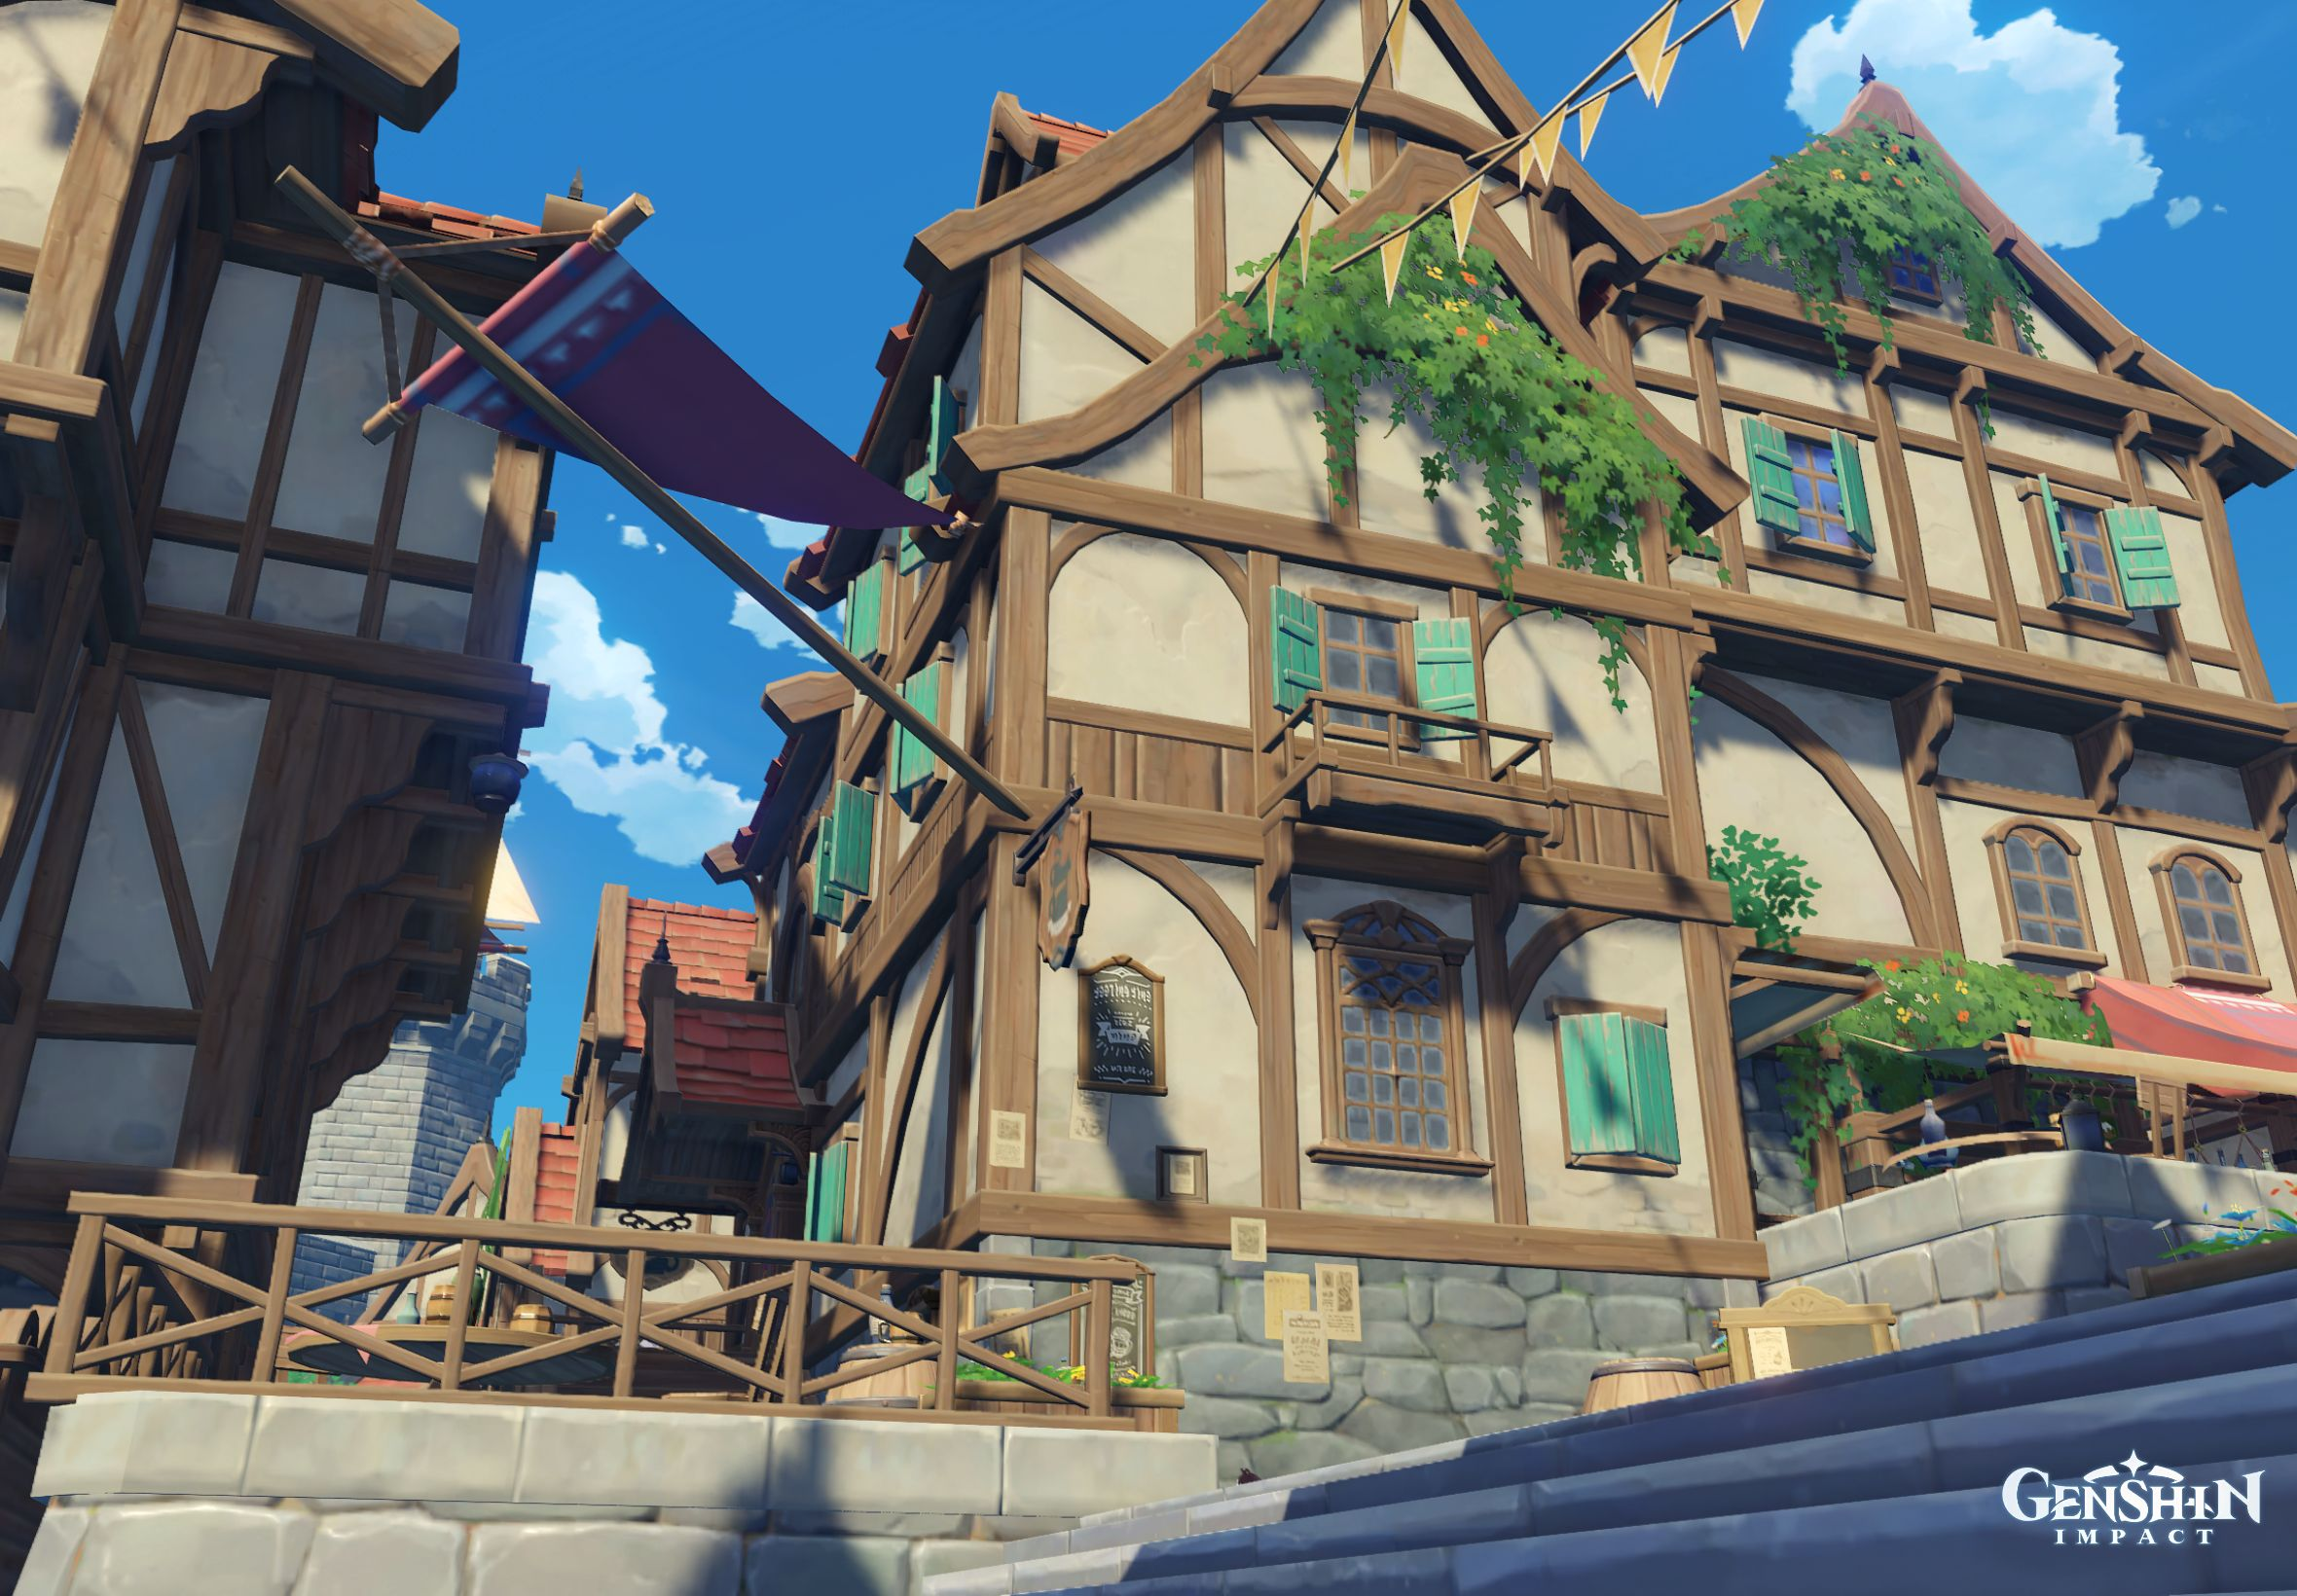
\includegraphics[scale=0.15]{cattail.jpg} \\
  \small{猫尾酒馆}
\end{center}

